\documentclass[a4paper,12pt]{article}

% -------------------------------------------------
% Pacchetti essenziali
% -------------------------------------------------
\usepackage[utf8]{inputenc}
\usepackage[T1]{fontenc}
\usepackage{lmodern}
\usepackage{amsmath,amsfonts,amssymb}
\usepackage{graphicx}
\usepackage{listings,xcolor}
\usepackage{enumitem}
\usepackage{hyperref}
\usepackage{tikz}
\usepackage[official]{eurosym}
\usepackage{float}
\hypersetup{
	colorlinks=true,
	linkcolor=blue,
	urlcolor=blue,
	citecolor=blue
}
% -------------------------------------------------

\begin{document}
	
	% ---------- Frontespizio (pag. 1) ----------------
\title{\textbf{Stochastic Optimization}\\
	\vspace{0.5em}\huge\textbf{Report}
	\author{
		Di Battista Simona — 302689%\\
		\and
		Rostagno Andrea — 349152\\
	}
	
	\vspace{0.5cm}
	\large Assignment 2024/25}
%%\date{\today}
\maketitle
\thispagestyle{empty}   % (facoltativo) niente numero in frontespizio
\newpage                % <-- salto di pagina: l’indice parte da qui

	
	% ---------- Indice (pag. 2) ----------------------
	\pagenumbering{roman}   % numeri romani per indice (i, ii, iii…)
	\tableofcontents
	\newpage                % nuovo salto: inizia il testo
	
	% ---------- Testo principale (da pag. 3) ---------
	\pagenumbering{arabic}  % riparte da 1 con numeri arabi
	
	% =================================================
	\section{Introduction}
	Stochastic optimization addresses decision-making problems under uncertainty, where parameters not known in advance are modeled as random variables. Unlike deterministic optimization, stochastic optimization aims to identify optimal decisions by considering the probabilistic distribution of future scenarios. In this project, we specifically focus on two classical stochastic problems: the Newsvendor Problem and the Assemble-to-Order (ATO) problem. The Newsvendor Problem involves determining the optimal quantity of newspapers to order under uncertain demand, to maximize expected profits. In contrast, the ATO problem addresses component inventory and assembly decisions to satisfy uncertain demand for multiple products.
	
	To analyze these problems, scenarios were generated through a predefined scenario generation code provided beforehand. Subsequently, to reduce computational complexity, were applied two scenario reduction methods: 
	\begin{itemize}
	\item $K$-means clustering; 
	\item an heuristic method, based on Wasserstein distance.
	\end{itemize}
	 Finally, were compared the results to evaluate effectiveness and stability of each strategy.
	
	\section{Problems explanation}
	
	In this section, are presented the two stochastic optimization problems analyzed in this report: the Newsvendor Problem and the Assemble-to-Order (ATO) Problem. Both are classical examples of two-stage stochastic programs, characterized by decisions that must be made before uncertain demand is revealed. First each problem is introduced and mathematically formulated, then a schematic representations is given to aid understanding. Finally, these problems are solved and analyzed, using different scenario generation and reduction methods.
	
	\subsection{Newsvendor Problem}
	
	The newsvendor problem is a classical example in stochastic optimization used to determine the optimal inventory level when demand is uncertain. In our analysis, a vendor must decide the optimal number of newspapers to buy at the beginning of a day, without knowing the exact daily demand, with the goal of maximizing total expected profit.
	
	\subsubsection{Problem Formulation}
	
	Formally, the problem is formulated as follows:
	\[
	\max_{x} \mathbb{E}[p\min(D(\omega), x) - cx]
	\]
	
	with:
	\begin{itemize}
		\item \( x \): decision variable representing the number of newspapers to buy;
		\item \( D(\omega) \): a random variable modeling daily demand, characterized by discrete scenarios \( d_s \), each with probability \( \pi_s \);
		\item \( p \): selling price per newspaper.
		\item \( c \): cost per newspaper.
	\end{itemize}
	\vspace{0.20cm}

	In our specific implementation:
	
	\begin{itemize}
		\item \( c = 1 \);
		\item \( p = 10 \).
		%\item $D(\omega)$ $\sim$ $N(25,\sqrt{200})$, whose samples are generated using the provided scenario tree code, and rounded to integer numbers.
	\end{itemize}
	
	\subsubsection{Optimization Model}
	
	The model is implemented using the following integer linear programming formulation:
	\[
	\begin{aligned}
		\max & \quad p \sum_{s \in S} \pi_s y_s - c x \\
		\text{s.t.} & \quad y_s \leq x, & \forall s \in S \\
		& \quad y_s \leq d_s, & \forall s \in S \\
		& \quad x, y_s \geq 0 \quad \text{and integers}, & \forall s \in S
	\end{aligned}
	\]
	
\noindent	where \( y_s \) represents the actual number of newspapers sold if scenario \( s \) is realized.
	
	\subsection{Assemble-to-Order (ATO) Problem}
	
	The Assemble-to-Order (ATO) problem addresses decision-making in manufacturing systems, where final products are assembled from a set of pre-produced components once customer orders are realized. This two-stage stochastic program involves:
	\begin{itemize}
		\item \textbf{first stage}: decide the quantities of components to produce.
		\item \textbf{second stage}: determine the assembly quantities of final products, once demand is known.
	\end{itemize}
	
	\subsubsection{Problem Formulation}
	
	The mathematical formulation of the ATO problem is given by:
	\[
	\begin{aligned}
		\max & \quad -\sum_{i \in \mathcal{I}} C_i x_i + \mathbb{E}\left[\sum_{j \in \mathcal{J}} P_j y_j(\omega)\right] \\
		\text{s.t.} & \quad \sum_{i \in \mathcal{I}} T_{im} x_i \leq L_m, & \forall m \in \mathcal{M} \\
		& \quad y_j(\omega) \leq d_j(\omega), & \forall j \in \mathcal{J}, \forall \omega \in \Omega \\
		& \quad \sum_{j \in \mathcal{J}} G_{ij} y_j(\omega) \leq x_i, & \forall i \in \mathcal{I}, \forall \omega \in \Omega \\
		& \quad x_i, y_j(\omega) \geq 0, & \forall i \in \mathcal{I}, j \in \mathcal{J}, \omega \in \Omega
	\end{aligned}
	\]
	
	with:
		
		\begin{itemize}
		\item $x_i$: decision variable representing the amount of component $i \in \mathcal{I}$ (set of components) to produce;
		\item $y_j(\omega)$: amount of item $j \in \mathcal{J}$ (set of final items) assembled after demand realization;
		\item $d_j(\omega)$: stochastic demand for item $j$ in scenario $\omega \in \Omega$.
		\item $C_i$: cost of component $i$;
		\item $P_j$: selling price of item $j$;
		\item $L_m$: availability of machine $m$;
		\item $T_{im}$: time required to produce component $i$ on machine $m$;
		\item $G_{ij}$: amount of component $i$ required to assemble item $j$ (Gozinto factor);
		\item $\mathcal{M}$: set of machines.
			
	\end{itemize}
\vspace{0.20cm}	
In our specific implementation, we considered the example of the pizza maker, with six hours of work available, two different types of pizzas to be able to produce and the following ingredients on hand: dough, tomato sauce, vegetables. The parameters in the optimization problem are set as follows:  
		\begin{itemize}
		\item $C = [1, 1, 3]$.
		\item $P = [6, 8.5]$.
		\item $T = [0.5, 0.25, 0.25]$.
		\item $L = 6.0$ hours.
		\item Gozinto matrix: $G = \begin{bmatrix} 1 & 1 \\ 1 & 1 \\ 0 & 1 \end{bmatrix}$.
	\end{itemize}
	
	\noindent These parameters and constraints form the basis of our computational experiments. 
	
	\section{The class \texttt{ScenarioTree}}
	
	The scenario tree is a fundamental tool in stochastic optimization used to represent and manage uncertainty through a structured set of possible future scenarios. In this study, scenario trees are generated using a two-step process involving initial probabilistic models and a specialized Python class called \texttt{ScenarioTree}.
	
	\subsection{Initial Probabilistic Model}
	
	Initially, scenarios are generated using a stochastic model defined by the class \texttt{EasyStochasticModel}. This class uses a multivariate normal distribution characterized by specified averages and variances; a certain number of scenarios are simulated according to the probability distribution
	
	\[
	\text{Obs} \sim \mathcal{N}(\mu, \Sigma)
	\]
	
	which parameters depend on the problem under consideration.	
			
	\subsection{Scenario Tree Generation}
	
	The \texttt{ScenarioTree} class is responsible for constructing and managing the tree structure. The tree is built iteratively, where each node generates child nodes according to the stochastic model described above. Each node has attributes:
	
	\begin{itemize}
		\item \textbf{obs}: observation values at the node.
		\item \textbf{prob}: conditional probability of reaching this node from its parent.
		\item \textbf{path\_prob}: cumulative probability from the root node to the current node.
	\end{itemize}
	
	Formally, for each node at stage $t$, child nodes are generated based on:
	
	\[
	\text{obs}^{(t+1)}_j \sim \text{StochModel}\bigl(\text{obs}^{(t)}\bigr), \quad j=1, \dots, \text{branching\_factor}_t
	\]
	
	The tree generation continues until the predefined depth (planning horizon) is reached, creating a comprehensive structure of all possible demand outcomes and associated probabilities.\\
	
	\noindent The resulting scenario tree can be visualized graphically, clearly illustrating the branching structure, node values, and probabilities. This visual aid significantly enhances the interpretation of how uncertainty evolves over time and assists in understanding the implications of different scenario reduction methods presented later in the report.
	
	
	\section{Results with all scenarios}
	
	In this section, are reported the results obtained by solving the stochastic optimization problem considering the full set of demand scenarios, without applying any reduction technique. This approach provides a benchmark solution, capturing the entire variability of the underlying random variables. The outcomes presented here will be useful as a reference for evaluating the accuracy and computational efficiency of the scenario reduction methods discussed in the following sections.
	
	\subsection{Newsvendor Problem}
	
	The following results summarize the optimization outcomes of the Newsvendor problem when considering all initially generated scenarios. From an initial root, 20 nodes sampled from a multivariate normal of size 50 were generated; each node was generated from the following distribution: 
	
	\[
	\mathcal{N}_{50}(\mu, \Sigma),
	\]
	
	 with $\mu = [25,\dots,25]$ and covariance matrix $\Sigma = 200 * I_{50}$. The code generates 20 samples of size 50 to obtain 20 realizations of the expected value of profit, in order to calculate statistics and draw results and conclusions about the solution of the problem.
	 The choice to place the number of scenarios equal to 50 was related to the use of a limited Gurobi license, while the choice of $\mu$ and $\Sigma$ parameters was dictated by the possibility of generating data that encapsulated some variability.
	\noindent Of course, the scenario tree generated through this procedure returns demand values as floating-point numbers. However, since the Newsvendor problem inherently deals with discrete units (we are talking about newspapers), these continuous observations must be rounded to the nearest integer and constrained to be non-negative, ensuring practical and realistic demand scenarios. This rounding and aggregation procedure is implemented in the code using the provided \texttt{aggregate\_discrete\_demands} function, which combines scenarios with identical integer demands, summing their probabilities.\\
	
	\noindent 

\textcolor{red}{The resulting distinct integer demands and corresponding probabilities are summarized in the table below:}	
	
	\begin{table}[htbp]
		\centering
		\footnotesize % rende il testo più piccolo
		\label{tab:newsvendor-general}
		\renewcommand{\arraystretch}{1.1}
		\begin{tabular}{|@{\hskip 2pt}p{1.5cm}@{\hskip 2pt}|@{\hskip 2pt}p{2.0cm}@{\hskip 2pt}||@{\hskip 2pt}p{1.5cm}@{\hskip 2pt}|@{\hskip 2pt}p{2.0cm}@{\hskip 2pt}||@{\hskip 2pt}p{1.5cm}@{\hskip 2pt}|@{\hskip 2pt}p{2.0cm}@{\hskip 2pt}|}
			\hline
			\textbf{Demand (d)} & \textbf{Probability ($\pi$)} & \textbf{Demand (d)} & \textbf{Probability ($\pi$)} & \textbf{Demand (d)} & \textbf{Probability ($\pi$)} \\
			\hline
			0 & 0.06 & 19 & 0.08 & 39 & 0.06 \\
			1 & 0.02 & 21 & 0.02 & 42 & 0.02 \\
			4 & 0.02 & 23 & 0.04 & 43 & 0.02 \\
			5 & 0.02 & 24 & 0.02 & 46 & 0.04 \\
			7 & 0.02 & 25 & 0.04 & 48 & 0.02 \\
			10 & 0.02 & 29 & 0.04 & 56 & 0.04 \\
			12 & 0.02 & 30 & 0.04 & 57 & 0.02 \\
			13 & 0.06 & 31 & 0.02 & 59 & 0.02 \\
			14 & 0.02 & 33 & 0.02 & \textbf{Total} & \textbf{1.00} \\
			15 & 0.04 & 35 & 0.04 & & \\
			16 & 0.04 & 38 & 0.04 & & \\
			17 & 0.02 & & & & \\
			\hline
		\end{tabular}
		\caption{Discrete demand values and aggregated probabilities used in the Newsvendor model.}
	\end{table}
	
	
\textcolor{red}{Given these discrete demand scenarios, the optimization model solved through the Newsvendor model implementation yielded the following results:}	
	
	\begin{itemize}
		\item \textbf{Optimal quantity of newspapers to order:} $x^* = 48$;
		\item \textbf{Maximum expected profit:} 202.00\,€.
	\end{itemize}
	\newpage
	The plot illustrating the scenario tree (Figure~\ref{fig:scenariotree-plot}) visually depicts the generated demand values, their probabilities, and the structure of uncertainty, showcasing clearly the equal probabilities (0.02 each) initially assigned to the generated scenarios before aggregation.
	
	\begin{figure}[htbp]
		\centering
		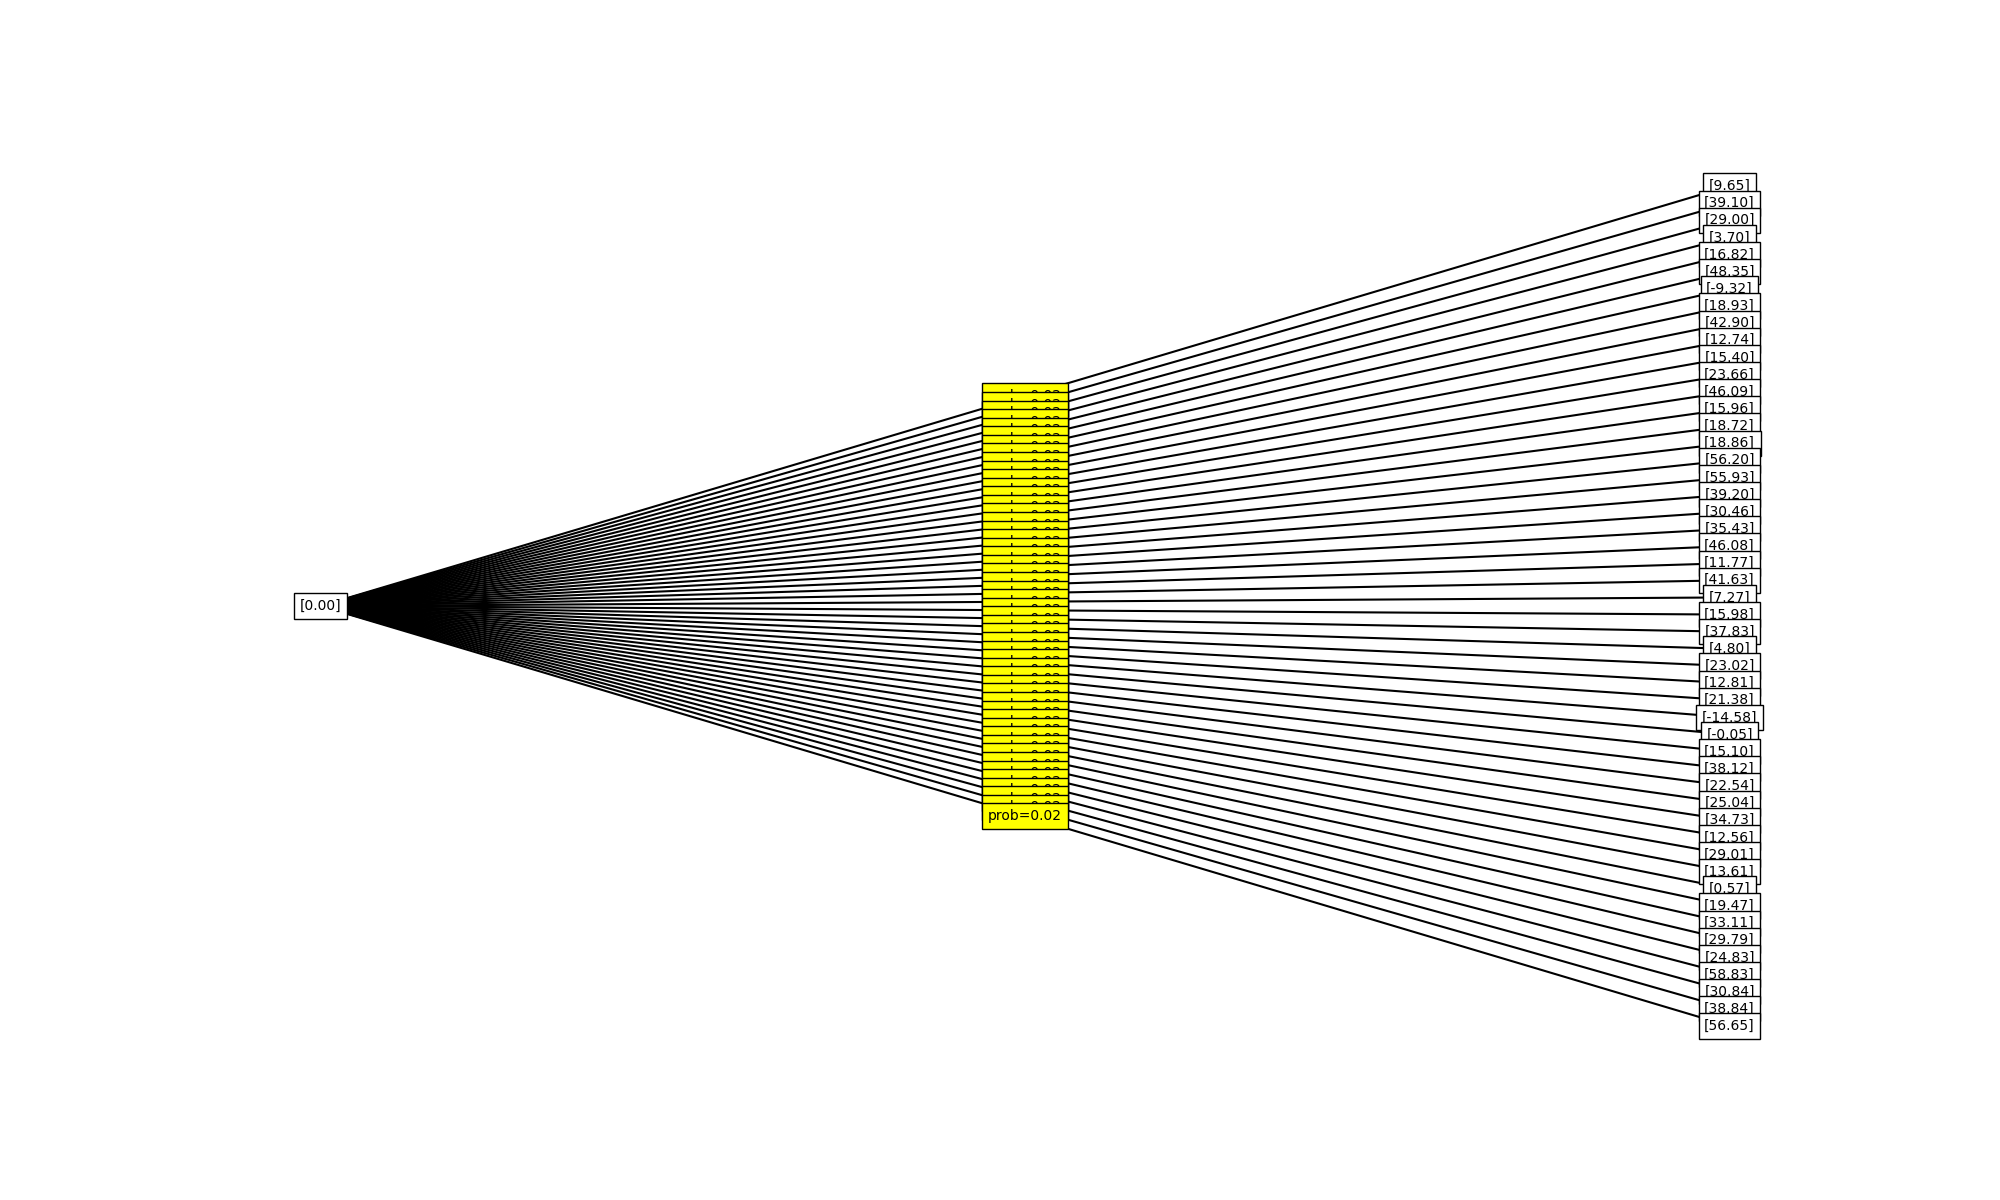
\includegraphics[width=1\textwidth]{../immagini/scenariNV.png}
		\caption{Visualization of the generated scenario tree for the Newsvendor problem (50 cases).}
		\label{fig:scenariotree-plot}
	\end{figure}
	
	This scenario tree clearly highlights the transformation from continuous demand values (floating points) generated by the stochastic model to the practical integer demands necessary for the Newsvendor optimization. Such transformation, performed via aggregation, ensures consistency with the discrete nature of the problem and simplifies computational processing while maintaining scenario integrity.
	
	\newpage
	\subsection{ATO Problem}
	
	This subsection presents the results of the Assemble-to-Order (ATO) optimization model using the complete set of scenarios generated by our stochastic model.\\
	
	\noindent In this case 20 sets of observations sampled from a multivariate normal of size 50 were generated for each type of pizza considered in the problem. Specifically, the parameters $\mu_{1} = 90, \Sigma_{1} = 200 * I_{50}$ were considered for the first typology, while the parameters $\mu_{2} = 100, \Sigma_{2} = 2000 * I_{50}$ were considered for the second one. Even in this case this procedure is used to obtain samples of the expected value of profit, to calculate statistics useful for drawing conclusions about the problem. The choice to place the number of scenarios equal to 50 was related to the use of a limited Gurobi license, while the choice of $\mu$ and $\Sigma$ parameters was dictated by the possibility of generating data that encapsulated some variability. The generated demands, initially provided as continuous values from a multivariate normal distribution, must be discretized to integer values due to the practical constraints of real-world production systems. Specifically, demands are rounded to the nearest multiple of ten, ensuring realistic and manageable scenarios. This procedure is implemented by the provided function \texttt{aggregate\_vectorial\_demands}, which aggregates the probabilities of scenarios with identical discretized demands. 
	
	\textcolor{red}{The final distinct demands and their probabilities are reported in Table~\ref{tab:ato-general-results}:}
		
	\begin{table}[htbp]
		\centering
		\footnotesize
		\label{tab:ato-general-results}
		\renewcommand{\arraystretch}{1.1}
		\begin{tabular}{|@{\hskip 2pt}p{3.2cm}@{\hskip 2pt}|@{\hskip 2pt}p{1cm}@{\hskip 2pt}||@{\hskip 2pt}p{3.2cm}@{\hskip 2pt}|@{\hskip 2pt}p{1cm}@{\hskip 2pt}||@{\hskip 2pt}p{3.2cm}@{\hskip 2pt}|@{\hskip 2pt}p{1cm}@{\hskip 2pt}|}
			\hline
			\textbf{Demand (Item 1, 2)} & \textbf{$\pi$} &
			\textbf{Demand (Item 1, 2)} & \textbf{$\pi$} &
			\textbf{Demand (Item 1, 2)} & \textbf{$\pi$} \\
			\hline
			\texttt{[60, 190]}  & 0.02 & \texttt{[80, 270]} & 0.02 & \texttt{[100, 100]} & 0.02 \\
			\texttt{[70, 160]}  & 0.04 & \texttt{[80, 280]} & 0.02 & \texttt{[100, 150]} & 0.02 \\
			\texttt{[80, 120]}  & 0.02 & \texttt{[90, 90]}   & 0.02 & \texttt{[100, 160]} & 0.04 \\
			\texttt{[80, 140]}  & 0.04 & \texttt{[90, 150]}  & 0.02 & \texttt{[100, 180]} & 0.04 \\
			\texttt{[80, 150]}  & 0.02 & \texttt{[90, 160]}  & 0.02 & \texttt{[100, 200]} & 0.04 \\
			\texttt{[80, 170]}  & 0.02 & \texttt{[90, 170]}  & 0.02 & \texttt{[100, 210]} & 0.02 \\
			\texttt{[80, 190]}  & 0.04 & \texttt{[90, 180]}  & 0.04 & \texttt{[100, 230]} & 0.02 \\
			\texttt{[80, 210]}  & 0.04 & \texttt{[90, 200]}  & 0.02 & \texttt{[100, 260]} & 0.02 \\
			\texttt{[80, 220]}  & 0.02 & \texttt{[90, 220]}  & 0.04 & \texttt{[100, 270]} & 0.04 \\
			\texttt{[80, 240]}  & 0.02 & \texttt{[90, 240]}  & 0.04 & \texttt{[110, 170]} & 0.02 \\
			\texttt{[80, 250]}  & 0.04 & \texttt{[90, 290]}  & 0.02 & \texttt{[110, 240]} & 0.04 \\
			\texttt{[80, 260]}  & 0.04 & \texttt{[90, 310]}  & 0.02 & \texttt{[110, 300]} & 0.02 \\
			\hline
			\multicolumn{5}{|r|}{\textbf{Total}} & \textbf{1.00} \\
			\hline
		\end{tabular}
		\caption{Demand scenarios and probabilities for the ATO problem (without scenario index).}
	\end{table}
	

	\textcolor{red}{Based on these discrete scenarios, we solved the ATO model, obtaining the optimal quantities of components to produce:}
	
	\begin{itemize}
		\item Component 0 (Dough): \(8.00\);
		\item Component 1 (Tomato Sauce): \(8.00\);
		\item Component 2 (Vegetables): \(0.00\).
	\end{itemize}
	
	The optimal solution yields a maximum expected profit of \(32.00\)\,€.
	
	\newpage
 The scenario tree visualization (Figure~\ref{fig:ato-scenariotree}) clearly illustrates the initial stochastic process, from continuous to discrete demands. Initially generated continuous values from the stochastic model undergo a rounding process to ensure integer values compatible with the practical nature of the ATO model.
	
	\begin{figure}[htbp]
		\centering
		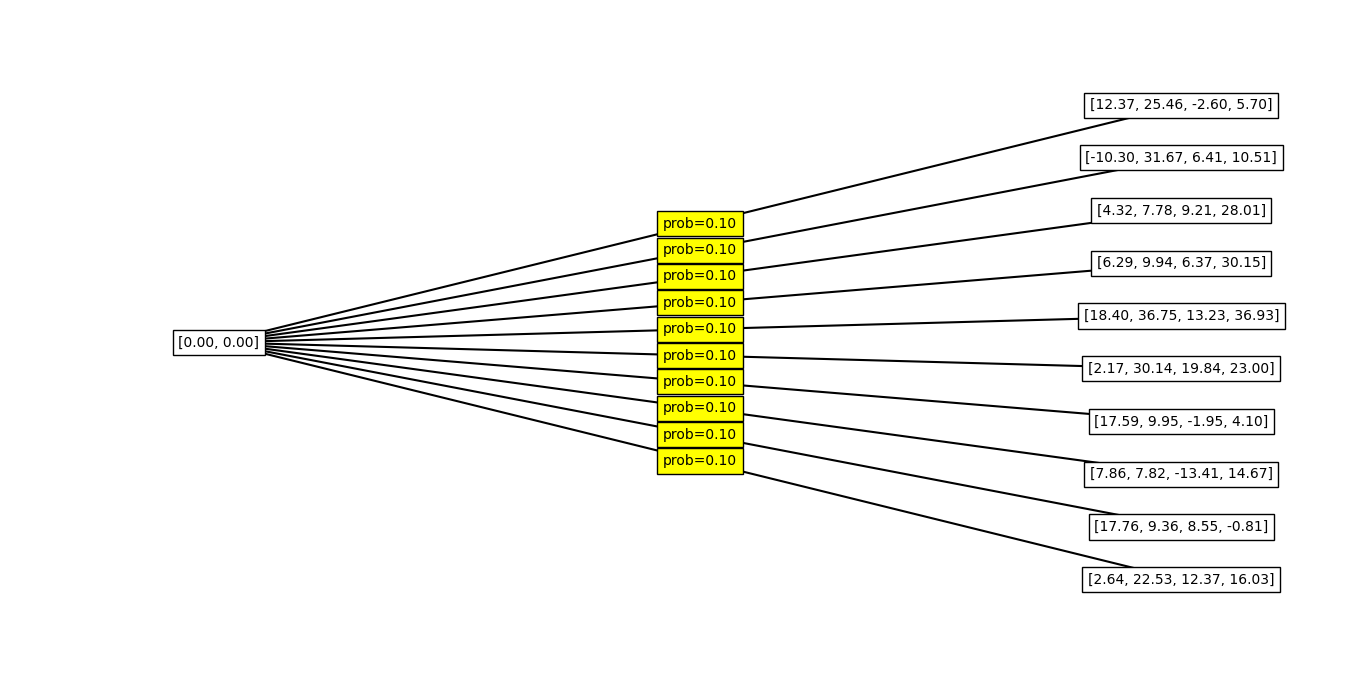
\includegraphics[width=1\textwidth]{../immagini/scenariATO.png}
		\caption{Visualization of the generated scenario tree for the ATO problem.}
		\label{fig:ato-scenariotree}
	\end{figure}
	
	\noindent This discretization approach provides a realistic representation of demand uncertainty, facilitating the optimization procedure while maintaining the relevance and practicality of the obtained solutions.
	
	
	\section{Results with K-means reduction}
	
	In this section, we present the results obtained by applying the K-means clustering method to reduce the number of scenarios and computational complexity generated in both the Newsvendor and Assemble-to-Order (ATO) problems. K-means is a clustering algorithm that partitions the original set of scenarios into \(k\) clusters by minimizing the weighted sum of squared distances between scenario values and their respective cluster centroids. Specifically, each original scenario is assigned to a cluster based on its proximity to the cluster's centroid, taking into account the scenario probabilities as weights. After the clustering process, the centroids become representative of the reduced scenarios, and the probabilities of these scenarios are recalculated by summing the probabilities of all original scenarios within each cluster.
	
	\noindent K-means clustering were implemented to reduce the number of original scenarios generated for both problems. The algorithm was applied to each of the 20 samples, to reduce the numerosity of each sample from 50 to $k$, with $k \in [1,15]$. The upper bound of the interval was chosen such that the number of clusters obtained was significantly smaller than the original number of scenarios. Each resulting cluster, in fact, is represented by its centroid, which acts as a reduced scenario, with the new scenario probability obtained by summing the probabilities of the original scenarios assigned to that cluster. Furthermore, for each of the 20 samples, the SSE trend graph was plotted to identify the appropriate number of points (clusters) to represent each initial set, according to the algorithm.\\
	
	\noindent Below, we present detailed analyses of the performance of this scenario reduction method in the two considered optimization problems.
	
	\subsection{Newsvendor Problem}
	
	
	
	\textcolor{red}{The reduced scenarios obtained are listed in Table~\ref{tab:kmeans-nv-results}:}
	
	\[
	\begin{array}{ccc}
		\hline
		\text{Cluster} & \text{Demand ($d_{s}$)} & \text{Probability (\(\pi_{s}\))} \\
		\hline
		1 & 3 & 0.16 \\
		2 & 18 & 0.40 \\
		3 & 34 & 0.26 \\
		4 & 45 & 0.10 \\
		5 & 57 & 0.08 \\
		\hline
		\text{Total} & & 1.00 \\
		\hline
	\end{array}
	\]
	\label{tab:kmeans-nv-results}
	
	By solving the Newsvendor optimization model with these reduced scenarios, we obtained the following results:
	
	\begin{itemize}
		\item Optimal order quantity: \( x^* = 45 \); newspapers
		\item Maximum expected profit: \(201.20\)\,€.
	\end{itemize}
	
	These results demonstrate how scenario reduction via K-means effectively simplifies the scenario representation while preserving the essential characteristics needed to achieve reliable decision-making outcomes in stochastic optimization contexts.
	
	\begin{figure}[H]
		\centering
		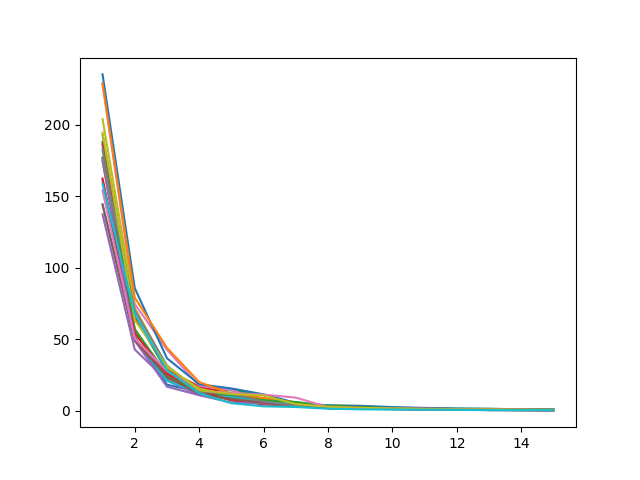
\includegraphics[width=0.8\textwidth]{../immagini/sseNV.png}
		\caption{SSE trend graph for $k \in [1,15]$ in case of Newsvendor problem. The figure shows that the appropriate number of points to which to reduce the numerosity of each set is around 3 and 4.}
		\label{fig:sse-nv}
	\end{figure}
	
	
	\newpage
	\subsection{ATO Problem}
	
	In this subsection, we present the results obtained for the Assemble-to-Order (ATO) problem after applying scenario reduction via K-means clustering, to identify representative scenarios in a two-dimensional space (corresponding to the two final products). The final reduced scenarios and their associated probabilities are shown in Table~\ref{tab:kmeans-ato-results}:
	
	\[
	\begin{array}{ccc}
		\hline
		\text{Scenario} & \text{Demand [Item 1, Item 2]} & \text{Probability (\(\pi\))} \\\\
		\hline
		1 & [90, 130] & 0.16 \\\\
		2 & [90, 170] & 0.30 \\\\
		3 & [90, 220] & 0.30 \\\\
		4 & [90, 260] & 0.18 \\\\
		5 & [100, 300] & 0.06 \\\\
		\hline
		\text{Total} & & 1.00 \\\\
		\hline
	\end{array}
	\]
	\label{tab:kmeans-ato-results}
	
	After solving the ATO model using these reduced scenarios, we obtained the following optimal component production plan:
	
	\begin{itemize}
		\item Component 0 (Dough): \(8.00\);
		\item Component 1 (Tomato Sauce): \(8.00\);
		\item Component 2 (Vegetables): \(0.00\).
	\end{itemize}
	
	The resulting maximum expected profit is \(32.00\)\,€, exactly matching the value obtained with the full set of scenarios. This indicates that the scenario reduction via K-means preserved the essential characteristics of the demand distribution, allowing us to significantly reduce the problem size while maintaining optimality in the solution.
	
	\begin{figure}[H]
		\centering
		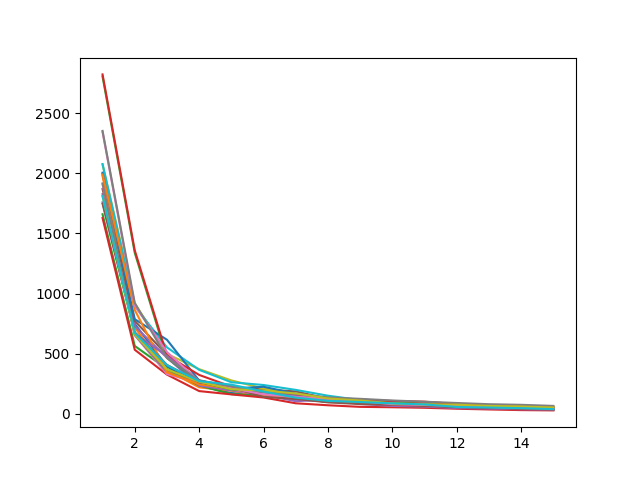
\includegraphics[width=0.8\textwidth]{../immagini/sseATO.png}
		\caption{SSE trend graph for $k \in [1,15]$ in case of ATO problem. The figure shows that the appropriate number of points to which to reduce the numerosity of each set is around 3 and 4.}
		\label{fig:sse-ato}
	\end{figure}
	
	
	\section{Results with Wasserstein distance--based reduction}
	
	In this section, we present the scenario reduction method based on the Wasserstein distance, as applied to both the Newsvendor and Assemble-to-Order (ATO) problems. The Wasserstein distance, also known as the Earth Mover's Distance, is a mathematical metric used to quantify the dissimilarity between two probability distributions on a given metric space. In the context of scenario reduction, it measures the minimum "cost" required to transform the original probability distribution of scenarios into a reduced one, where the "cost" is defined as the amount of probability mass to move times the distance it is moved.
	
	Formally, let $\mu = (\mu_1, \ldots, \mu_m)$ and $\nu = (\nu_1, \ldots, \nu_n)$ be two discrete probability distributions on points $x_1, \ldots, x_m$ and $y_1, \ldots, y_n$. The $p$-Wasserstein distance is defined as:
	\[
	W_p(\mu, \nu) = \left( \min_{\gamma \in \Gamma(\mu, \nu)} \sum_{i=1}^m \sum_{j=1}^n \|x_i - y_j\|^p \gamma_{ij} \right)^{1/p}
	\]
	where $\gamma_{ij}$ is the transport plan representing the amount of mass moved from $x_i$ to $y_j$, and $\Gamma(\mu, \nu)$ is the set of admissible transport plans (satisfying mass conservation constraints).
	
	In our scenario reduction approach, we use an exact mixed-integer programming (MILP) formulation to select a subset of $k$ representative scenarios from the original $m$ scenarios, such that the Wasserstein distance between the original and reduced distributions is minimized. The core optimization problem, implemented in our code, is as follows (for the unidimensional case):
	
	\[
	\begin{aligned}
		\min_{\gamma, z, \nu} \quad & \sum_{i=1}^m \sum_{j=1}^m c_{ij} \gamma_{ij} \\\\
		\text{s.t.} \quad
		& \sum_{j=1}^m \gamma_{ij} = \mu_i \qquad \forall i=1,\ldots,m \\
		& \sum_{i=1}^m \gamma_{ij} = \nu_j \qquad \forall j=1,\ldots,m \\
		& \nu_j \leq z_j \qquad \forall j=1,\ldots,m \\
		& \sum_{j=1}^m z_j = k \\
		& \sum_{j=1}^m \nu_j = 1 \\
		& z_j \in \{0,1\}, \quad \gamma_{ij}, \nu_j \geq 0
	\end{aligned}
	\]
	where:
	\begin{itemize}
		\item $c_{ij} = |x_i - x_j|^p$ is the cost of moving mass from scenario $i$ to scenario $j$ ($L^p$ norm);
		\item $\gamma_{ij}$ is the amount of probability mass transported from $i$ to $j$;
		\item $z_j$ is a binary variable indicating whether scenario $j$ is selected in the reduced set;
		\item $\nu_j$ is the probability assigned to scenario $j$ in the reduced distribution.
	\end{itemize}
	
	This model ensures that exactly $k$ scenarios are selected ($\sum_j z_j = k$), the reduced probabilities sum to 1, and the transportation of probability mass is minimized according to the cost matrix $C$. The same approach is extended to the multidimensional case (for ATO) using the appropriate vector norms for the cost computation.
	
	The Wasserstein reduction technique, by construction, selects scenarios that preserve the probabilistic structure of the original distribution as faithfully as possible, yielding a reduced scenario set that guarantees a minimal loss of information with respect to the original distribution. In the following subsections, we detail the results obtained by applying this method to our stochastic optimization problems.
	
	\subsection{Newsvendor Problem}
	
	For the Newsvendor problem, we applied the scenario reduction method based on the Wasserstein distance, which is designed to preserve the probabilistic structure of the original set of scenarios as closely as possible. The reduction is achieved by solving a mixed-integer linear program that selects $k = 5$ representative scenarios and reassigns the original probabilities to minimize the Wasserstein (Earth Mover's) distance between the original and reduced distributions.
	
	The resulting reduced scenarios and their associated probabilities are summarized in Table~\ref{tab:wass-nv-results}:
	
	\[
	\begin{array}{ccc}
		\hline
		\text{Scenario} & \text{Demand (d)} & \text{Probability (\(\pi\))} \\\\
		\hline
		1 & 1 & 0.14 \\\\
		2 & 16 & 0.32 \\\\
		3 & 29 & 0.26 \\\\
		4 & 42 & 0.20 \\\\
		5 & 57 & 0.08 \\\\
		\hline
		\text{Total} & & 1.00 \\\\
		\hline
	\end{array}
	\]
	\label{tab:wass-nv-results}
	
	By solving the Newsvendor optimization problem with this reduced scenario set, we obtained the following results:
	\begin{itemize}
		\item Optimal order quantity: $x^* = 42$ newspapers
		\item Maximum expected profit: $203.60$\,€
	\end{itemize}
	
	These results demonstrate the effectiveness of Wasserstein reduction: although the number of scenarios is significantly decreased, the essential statistical features of the original demand distribution are maintained. The reduced scenario set still allows the optimization model to find a solution that is both robust and close to the original optimal profit.
	\newpage
	\subsection{ATO Problem}
	
	In this subsection, we report the results for the Assemble-to-Order (ATO) problem using scenario reduction via the Wasserstein distance. The original multidimensional demand scenarios were reduced to $k=5$ representative scenarios by solving the exact MILP formulation that minimizes the Wasserstein distance, ensuring that the probabilistic and structural characteristics of the original distribution are preserved as faithfully as possible.
	
	The selected scenarios and their associated probabilities are summarized in Table~\ref{tab:wass-ato-results}:
	
	\[
	\begin{array}{ccc}
		\hline
		\text{Scenario} & \text{Demand [Item 1, Item 2]} & \text{Probability (\(\pi\))} \\\\
		\hline
		1 & [90, 160] & 0.30 \\\\
		2 & [90, 200] & 0.26 \\\\
		3 & [90, 240] & 0.24 \\\\
		4 & [90, 290] & 0.14 \\\\
		5 & [100, 100] & 0.06 \\\\
		\hline
		\text{Total} & & 1.00 \\\\
		\hline
	\end{array}
	\]
	\label{tab:wass-ato-results}
	
	Solving the ATO optimization problem with these reduced scenarios, we obtain the following optimal production plan:
	\begin{itemize}
		\item Component 0 (Dough): $8.00$
		\item Component 1 (Tomato Sauce): $8.00$
		\item Component 2 (Vegetables): $0.00$
	\end{itemize}
	
	The resulting maximum expected profit is $32.00$\,€, identical to the value obtained with the full set and the K-means reduction. This outcome highlights the robustness and accuracy of the Wasserstein-based scenario reduction, which manages to preserve the key features of the stochastic demand while significantly reducing computational complexity.
	
	\section{Efficiency}
	
	In this section, we compare the computational efficiency of the different scenario reduction methods applied to both the Newsvendor and ATO problems. We report and discuss the execution times of each algorithm, summarizing the results through graphical visualizations.
	
	\subsection{Newsvendor Problem}
	
	Figure~\ref{fig:timing-nv} shows the computational times required for the different phases of the Newsvendor problem, including both scenario reduction (K-means and Wasserstein) and the subsequent optimization with the reduced scenarios.
	
	\begin{figure}[htbp]
		\centering
		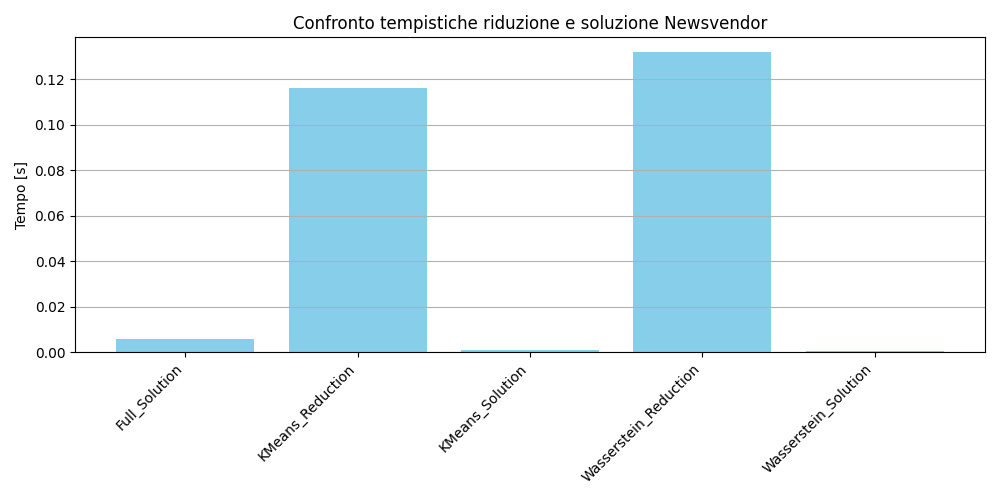
\includegraphics[width=1\textwidth]{../immagini/tempiNV.png}
		\caption{Comparison of computation times for scenario reduction and optimization (Newsvendor problem).}
		\label{fig:timing-nv}
	\end{figure}
	
	\begin{table}[htbp]
		\centering
		\caption{Execution times for scenario reduction and solution phases (Newsvendor problem).}
		\begin{tabular}{lc}
			\hline
			\textbf{Operation} & \textbf{Time [s]} \\
			\hline
			Full\_Solution         & 0.0058 \\
			KMeans\_Reduction      & 0.1160 \\
			KMeans\_Solution       & 0.0007 \\
			Wasserstein\_Reduction & 0.1318 \\
			Wasserstein\_Solution  & 0.0006 \\
			\hline
		\end{tabular}
		\label{tab:timing-nv}
	\end{table}
	
	
	
	From the chart, we observe that the time required to solve the full problem without reduction (\texttt{Full\_Solution}) is significantly lower than the time spent in the reduction phases (\texttt{KMeans\_Reduction} and \texttt{Wasserstein\_Reduction}), which dominate the total computational cost. Conversely, the actual optimization on the reduced scenario sets (\texttt{KMeans\_Solution} and \texttt{Wasserstein\_Solution}) is almost negligible in terms of time. 
	
	This result highlights that, for the Newsvendor problem with a moderate number of scenarios, the bottleneck is the reduction procedure itself—especially when using methods such as K-means or Wasserstein MILP—while the optimization stage becomes extremely fast once the scenario set is reduced. Therefore, the choice of the reduction algorithm and its implementation has a direct impact on the overall computational efficiency of the workflow.
	\newpage
	\subsection{ATO Problem}
	
	Figure~\ref{fig:timing-ato} reports the computational times for the different phases of the Assemble-to-Order (ATO) problem, including both the scenario reduction steps (K-means and Wasserstein) and the subsequent optimization using the reduced scenarios.
	
	\begin{figure}[htbp]
		\centering
		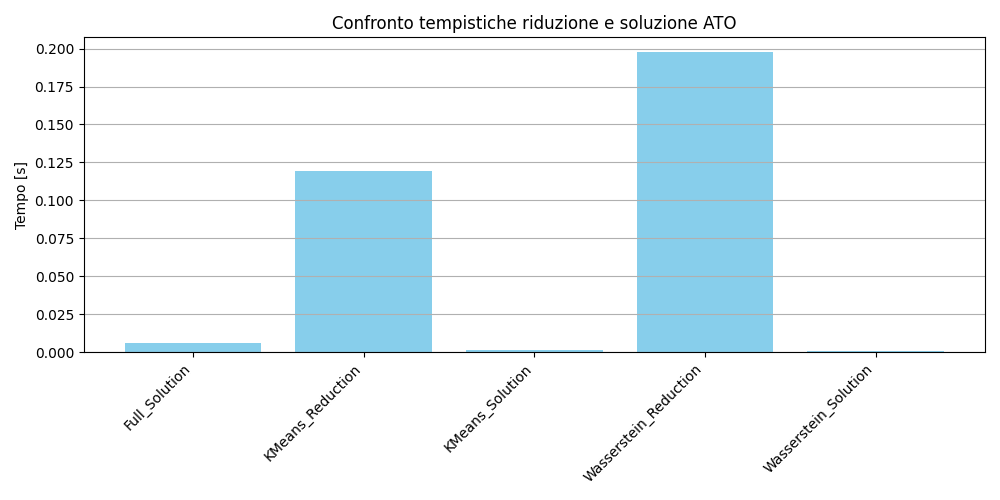
\includegraphics[width=1\textwidth]{../immagini/tempiATO.png}
		\caption{Comparison of computation times for scenario reduction and optimization (ATO problem).}
		\label{fig:timing-ato}
	\end{figure}
	
	\begin{table}[htbp]
		\centering
		\caption{Execution times for scenario reduction and solution phases (ATO problem).}
		\begin{tabular}{lc}
			\hline
			\textbf{Operation} & \textbf{Time [s]} \\
			\hline
			Full\_Solution         & 0.0059 \\
			KMeans\_Reduction      & 0.1195 \\
			KMeans\_Solution       & 0.0012 \\
			Wasserstein\_Reduction & 0.1975 \\
			Wasserstein\_Solution  & 0.0009 \\
			\hline
		\end{tabular}
		\label{tab:timing-ato}
	\end{table}
	
	
	As with the Newsvendor case, the time required for the scenario reduction phases (\texttt{KMeans\_Reduction} and \texttt{Wasserstein\_Reduction}) is substantially higher than the time needed to solve the full problem without reduction (\texttt{Full\_Solution}) or to solve the optimization problem on the reduced scenario sets (\texttt{KMeans\_Solution} and \texttt{Wasserstein\_Solution}), which are both negligible in terms of computational cost.
	
	It is particularly evident that the Wasserstein reduction, involving the solution of a mixed-integer programming problem in a multidimensional space, is the most computationally demanding step. However, once the reduced scenario set is obtained, the final optimization becomes extremely efficient. 
	
	This analysis confirms that, for moderate instance sizes, the major computational effort is concentrated in the scenario reduction phase—especially for methods based on mathematical programming—while the actual optimization benefits greatly from working on a smaller scenario set. Thus, efficiency considerations must take into account not only the quality of the reduced scenarios, but also the time required for the reduction procedure itself.
	
	\section{Discussion}
	
	The analyses presented in this report highlight important aspects regarding both the quality of solutions and the computational efficiency of different scenario reduction techniques when applied to the Newsvendor and Assemble-to-Order (ATO) problems.\\
	
	From a solution perspective, all scenario reduction methods—K-means and Wasserstein distance—were able to preserve the essential structure of the original problems. In both cases, the optimal decisions (order quantity for Newsvendor, component production plan for ATO) and the expected profit obtained with the reduced scenario sets were virtually identical to those derived from the full set of scenarios. This demonstrates the effectiveness of both K-means and Wasserstein-based reductions in maintaining solution quality while decreasing the scenario space.\\
	
	When considering computational efficiency, however, the results highlight important differences. The computational cost of the actual optimization, both for the full and reduced scenario sets, is negligible for both problems. The majority of the total computation time is instead spent on the scenarios reduction phase itself, with the Wasserstein MILP approach being the most time-consuming, especially for the multidimensional ATO case. K-means, while still significantly slower than the direct optimization, consistently requires less time than the Wasserstein-based reduction.\\
	
	\noindent Comparing the two problems, the trends remain similar: the scenario reduction phase dominates the total computational time--especially as the dimensionality of the problem increases--but both reduction methods succeed in dramatically simplifying the scenario set without any meaningful loss in solution quality. In summary, the choice of the reduction technique may be guided by the available computational resources and the problem's dimensionality: K-means offers faster execution and satisfactory accuracy for most practical purposes, while the Wasserstein approach is preferable when maximum fidelity to the original probability distribution is required, at the expense of increased computation time.
	
	\begin{table}[htbp]
		\centering
		\caption{Summary of optimal solutions and objective values for both Newsvendor and ATO problems.}
		\begin{tabular}{|l|l|c|c|c|}
			\hline
			\textbf{Problem} & \textbf{Method} & \textbf{\# Scenarios} & \textbf{Optimal Variable} & \textbf{Objective Value (€)} \\
			\hline
			Newsvendor & Full           & 31 & $x^* = 48$          & 202.00 \\
			Newsvendor & K-means        & 5  & $x^* = 45$          & 201.20 \\
			Newsvendor & Wasserstein    & 5  & $x^* = 42$          & 203.60 \\
			\hline
			ATO        & Full           & 36 & $x^* = [8,\,8,\,0]$ & 32.00  \\
			ATO        & K-means        & 5  & $x^* = [8,\,8,\,0]$ & 32.00  \\
			ATO        & Wasserstein    & 5  & $x^* = [8,\,8,\,0]$ & 32.00  \\
			\hline
		\end{tabular}
		\label{tab:summary-results}
	\end{table}
	
	\begin{table}[htbp]
		\centering
		\caption{Total computation times (reduction + solution) for each method and problem.}
		\begin{tabular}{|l|l|c|}
			\hline
			\textbf{Problem} & \textbf{Method} & \textbf{Total Time [s]} \\
			\hline
			Newsvendor & Full           & 0.0058 \\
			Newsvendor & K-means        & 0.1167 \\
			Newsvendor & Wasserstein    & 0.1324 \\
			\hline
			ATO        & Full           & 0.0059 \\
			ATO        & K-means        & 0.1207 \\
			ATO        & Wasserstein    & 0.1984 \\
			\hline
		\end{tabular}
		\label{tab:summary-times}
	\end{table}
	
	
\end{document}